\subsection{Training dynamics}
\label{sec:training-dynamics}

\begin{figure}[t]
  \centering
  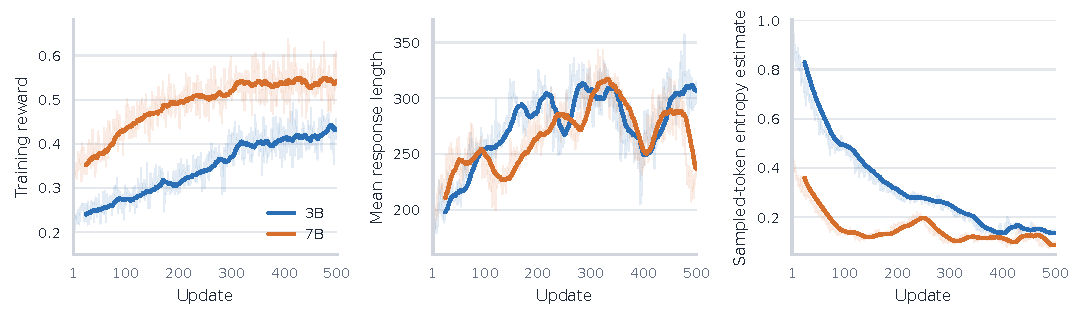
\includegraphics[width=\linewidth]{figures/training_dynamics.pdf}
  \caption{Optimization trajectories over 500 RLVR updates. Faint lines show
  per-update values, and solid lines show 25-update moving averages. Training
  reward is the bounded answer-and-format reward defined in
  Section~\ref{sec:experiments}. Response length is measured over sampled
  completions, and entropy is the sampled-token estimate recorded by the policy
  optimizer.}
  \label{fig:training-dynamics}
\end{figure}

Training reward increases at both model scales despite substantial
batch-to-batch variation. Averaged over the first and final 25 updates, mean
reward rises from 0.240 to 0.432 at 3B and from 0.353 to 0.542 at 7B. The 7B
model therefore begins and ends with higher reward, while both models exhibit
continued improvement throughout the single training pass.

The scales differ more clearly in their response-length trajectories. Mean
completion length increases from 198 to 308 tokens at 3B, compared with a
smaller increase from 211 to 237 tokens at 7B. Over the same intervals, the
sampled-token entropy estimate decreases from 0.829 to 0.137 at 3B and from
0.361 to 0.088 at 7B. Optimization therefore raises reward while making the
sampled token distributions more concentrated, without reducing the models to
shorter responses; both retain multi-hundred-token completions at the end of
training.
